\chapter{Künstliche Neuronale Netze}


\subsection{Renaissance der neuronalen Netze}\label{renaissance}


In den 80er Jahren sahen die großen Industrienationen in der Erforschung von KI einen Wettbewerbsvorteil, nachdem die Technologie durch den Einsatz von Expertensystemen (vgl \ref{appendix:expertensystem}) Einzug in die Wirtschaft gefunden hatte: So ermöglichte R1/XCON\footnote{
    das ``erste erfolgreiche kommerzielle Expertensystem`` [RN09:48, Abs. 1]
}  bei dem einsetzenden Unternehmen DEC (Digital Equipment Corporation) Einsparungen in Millionenhöhe [RN:48]: Die Domäne von R1 war die regelbasierte Konfiguration von VAX-11/780 Systemen nach Kundenanforderungen\footnote{
    siehe hierzu insb. [Mcd80] sowie [Hor90:63, Punkt 2]
}. Japan kündigte 1981 das 5th Generation Projekt [Gar19] an, einen Zehnjahresplan für den Aufbau ``intelligenter Computer`` [RN09:48, Abs. 2]\footnote{
    Zusammenfassend war das Ziel des 5th Generation Computer Systems (FGCS)-Projekt: ``Its ultimate goal is to develop integrated systems, both hardware and software, suitable for the major computer application in the nextdecade, identified by the Japanese as 'knowledge information processing'.`` in [Sha83:637, Anführungszeichen i.O. doppelt]
}, und in Großbritannien sorgte der Alvey-Report\footnote{
    \url{https://www.chilton-computing.org.uk/inf/literature/reports/alvey\_report/overview.htm} - empfohlene Massnahmen: \url{https://www.chilton-computing.org.uk/inf/literature/reports/alvey\_report/p008.htm} (beide abgerufen 31.08.2023)
} für eine Wiederaufnahme finanzieller Unterstützung, die durch den Lighthill-Report aufgehoben worden war [RN09:48, Abs. 2]\footnote{
    In Deutschland wird 1988 die DFKI GmbH (Deutsches Forschungszentrum für Künstliche Intelligenz) gegründet, eine ``wirtschaftsnahe Forschungseinrichtung`` auf ``dem Gebiet innovativer Softwaretechnologien auf der Basis von Methoden der Künstlichen Intelligenz`` (\url{https://www.dfki.de/fileadmin/user\_upload/DFKI/Medien/Ueber\_uns/DFKI\_im\_UEberblick/Unternehmensprofil/20210120\_DFKI\_Unternehmensprofil\_DE.pdf}, abgerufen 31.08.2023)
}.

Auch der technologische Fortschritt begünstigte das Wiederaufleben des Interesses an neuronalen Netzen, wie \textit{Olazaran} in Bezug auf die Modellierung paralleler Prozesse mit Hilfe von neuronalen Netzen anmerkt:

\blockquote[{[Ola96:644]}]{
    [...] increases in computer power and speed due to parallelism will undoubtedly favour neural net research.
}

denn mit den in den 80er Jahren verfügbaren Supercomputern und Parallelrechner\footnote{
    Auch \textit{Fausett} nennt bessere Rechenleistung als einen Grund für den erneuerten Enthusiasmus [Fau94:26]. Im Kontext der in diesem Kapitel vorgestellten mehrschichtigen Netzen und ihrem Konzept der versteckten Schichten ist nachvollziehbar, das mehr Rechenleistung den komplexen Verfahren entgegenkommt. \textit{Goodfellow, Bengio und Courville} gehen auf die Korrelation Modellgrösse und Anzahl der Nervenzellen in einem menschlichen Gehirn (vgl. Fussnote 15 in **Kapitel 1.2**) in [GBC18:24 ff.] ein
} erhält auch der Konnektionismus Auftrieb, der \textbf{neuronale Netze} als Grundlage hat [Dor91:15], und mit dem sich Modelle wieder mehr an den biologischen Vorbildern orientieren sollten\footnote{
    vgl. [RM87:43, Abs. 3] sowie [GBC18:18-19]}.


\subsection{Mehrschichtige neuronale Netze}

Bislang haben wir überwiegend künstliche Neuronen betrachtet, bei denen die Eingabe direkt mit der Ausgabe verbunden ist. Allerdings haben wir bereits für komplexe Boolesche Funktionen in Abschnitt~\ref{seq-mcpbool} gesehen, dass ein Verbund von mehreren MCP-Zellen in der Lage ist, auch Funktionen für nicht linear separable Daten zu modellieren. Hierzu hatten wir das MCP-Netz in zwei Schichten aufgeteilt, in denen die erste Schicht $X_1 := (\neg A \lor B)$ sowie $X_2 := (\neg B \lor A)$ und die zweite Schicht $X_1 \lor X_2$ formt, was nichts anderes als die disjunktive Normalform von XOR (Tabelle~\ref{tab:xor})ist.

Bei dem Rosenblatt-Perzeptron, das alleine nicht in der Lage ist, XOR zu erlernen, handelt es sich um ein \textbf{Einschichtiges neuronales Feedforward-Netz}.
Das bedeutet, dass es nur Eingabe und Ausgabe gibt und die Informationen ausschliesslich in Richtung Ausgang fliessen [RN09:848 ff.].

Allerdings ist auch ein \textbf{mehrschichtiges Perzeptron} (MLP, \textit{multi-layer perceptron}) [GBC18:6] in der Lage, nicht linear-separable Daten zu klassifizieren.
Ein MLP repräsentiert ein tiefes Feedforward-Netz, in dem die Eingabeschicht (\textbf{Input Layer}) und die Ausgabeschicht (\textbf{Output Layer}) über weitere Schichten von Neuronen (\textbf{hidden layer}) verbunden ist; die Neuronen in diesen Schichten implementieren Eingabe- und Aktivierungsfunktion und leiten ihre Berechnungen an die nächsten Zellen bis zu der Ausgabeschicht weiter. \textit{Murtagh} zeigt in [Mur91:184 ff.] die Modellierung von XOR anhand eines MLPs.

\begin{figure}[h]
    \centering
    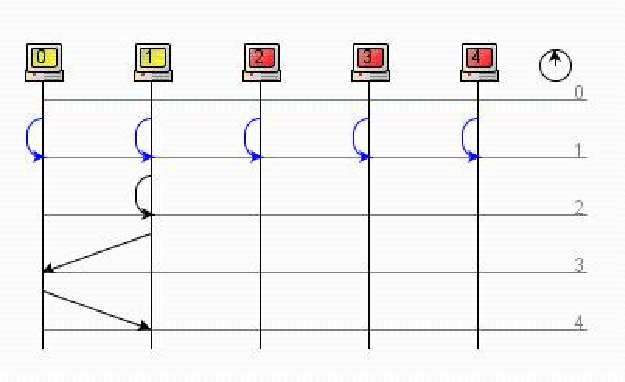
\includegraphics{images/p1ReadSeq.pdf}
    \caption{Skizzzierung eines mehrschichtigen neuronalen Feedforward-Netzwerks.}
    \label{fig-multilayerfeedforward}
\end{figure}



\subsection{Backpropagation}
In gleicher Arbeit ([Mur91:185 ff.]) zeigt \textit{Murtagh} ein MLP, das mittels \textbf{Backpropagation}\footnote{
    ``das meist genutzte neuronale Modell`` [Ert21:313, ``9.5 Der Backpropagation Algorithmus``]
} Daten klassifiziert, die keinen linearen Zusammenhang besitzen.
Der Algorithmus geht auf \textit{Rumelhart, Hinton und Williams} zurück, die in [RHW86a] eine Methode\footnote{
    ``The ability to create useful new features distinguishes back-propagation from earlier, simpler methods such as the perceptron-convergence procedure.`` [RHW86b:533]
} vorstellen, um berechnete Werte \textit{rückwärts} in das Netz einzuspeisen.
Hierbei wird für die Netzausgabe (\textit{forward pass}) ein Approximationsfehler berechnet, der als Basis für die Gewichtsänderungen beim rückwärtigen Lauf (\textit{backward pass}) bis zur ersten verborgenen Schicht genutzt wird.
Der Vorgang (forward pass, backward pass, forward pass...) wird so lange für alle Trainingsbeispiele wiederholt, bis die Gewichte sich nicht mehr ändern, oder eine andere Schranke (Epochen, Zeit) erreicht ist [Ert21:315]\footnote{
    ausführlicher Algorithmus in [RN09:853, Abbildung 18.24]
}.



Die mathematische Basis für Backpropagation ist das \textbf{Gradientenabstiegsverfahren}, das hilft, in einem neuronalen Netz Parameter für möglichst optimale Verlust-Werte (also geringe Fehler-Werte) zu finden [RN09:837] (s. Abbildung~\ref{fig-gradient})\footnote{
    ein kompakter Überblick zum Thema ``Optimierung auf Gradientenbasis`` findet sich in [GBC18:90 ff.]
}.  Ausserdem unterstützt die \textbf{Sigmoid}\footnote{
    \textit{sigmoid}: ``Sigma``, griechischer Buchstabe $\Sigma$, entspricht dem lateinischen ``S``; ``\textit{eidos}`` (griechisch) Form, Gestalt
}-Funktion (Gleichung~\ref{eq:gl-sigmoid} sowie Abbildung~\ref{fig-sigmoid}) als Aktivierungsfunktion\footnote{ ``Historisch wurde Backpropagation mit der Sigmoidfunktion implementiert.`` [Ert21:314, Fussnote 4] In Kapitel 9.5.3 (vgl. [RHW86a:329, (15)]). \textit{Ertel} fügt hinzu: ``Mittlerweile haben sich jedoch andere Funktionen als besser bewährt.`` In [Ert21:319] geht der Autor auf ``Probleme und Verbesserungen`` des mittlerweile über 30 Jahre alten Verfahrens ein. [GBC18:19]  stellt fest, dass Backpropagation der ``vorherrschende Ansatz für das Training tiefer Modelle`` (im Jahr 2018) ist.
}  aufgrund ihres nicht-linearen Charakters eine größere Klasse darstellbarer Funktionen und damit Lösungen für Probleme, die ein klassisches Perzeptron nicht lösen kann (vgl. [Ert 21:316])\footnote{
    In [RM86a] zeigen \textit{Rumelhart, Hinton und Williams} die Architektur eines mehrschichtigen neuronalen Netzes, das XOR über Backpropagation repräsentiert. Gleichzeitig grenzen sie in [RHW86b:536] ihr Modell vom biologischen Lernen ab: ``The learning procedure, in its current form, is not a plausible model of learning in brains``.
} \footnote{
    \textit{Ertel} weist darauf hin, dass die Klasse der darstellbaren Funktionen erhöht wird, wenn man für ein Perzeptron eine variable Sigmoid-Funktion verwendet [Ert21:316, Abs. 2]. Siehe hierzu auch ``Sigmoid-Perzeptron`` in [RN09:847]
}.\\

Sigmoid:
\begin{equation}
\sigma(x) = \begin{matrix}1 \\ \hline 1 + e^{-x}\end{matrix}
\label{eq:gl-sigmoid}
\end{equation}



\begin{figure}[h]
    \centering
    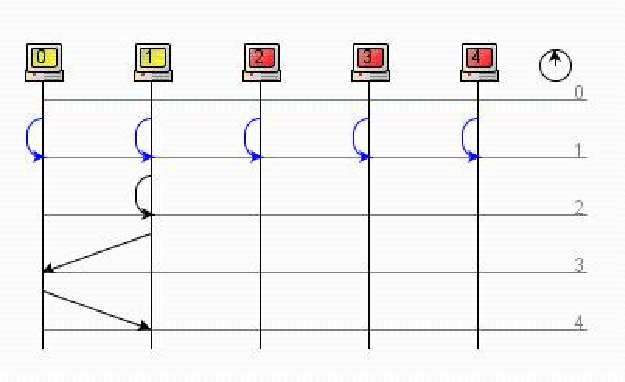
\includegraphics{images/p1ReadSeq.pdf}
    \caption{Ein Plot einer Sigmoid-Funktion}
    \label{fig-sigmoid}
\end{figure}


\begin{figure}[h]
    \centering
    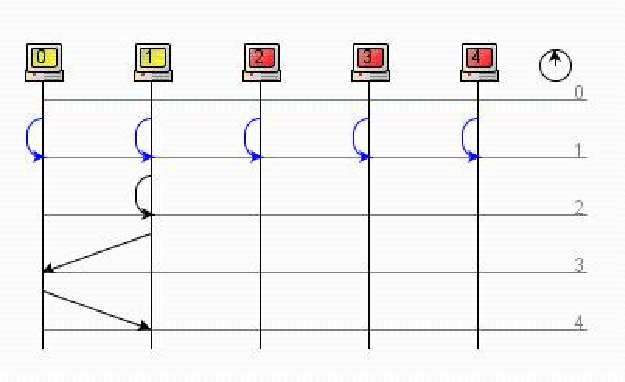
\includegraphics{images/p1ReadSeq.pdf}
    \caption{Skizzierung des Gradientenabtiegsverfahrens.}
    \label{fig-gradient}
    \small
    Informelle Darstellung des Gradientenabtiegsverfahrens. Die y-Achse repräsentiert die Anzahl der Fehler, die x-Achse den berechneten Gewichtsvektor in einem neuronalen Netz. Offensichtlich existiert in dem Netz ein optimaler Wert für w, der mittels Gradientenabstieg gefunden werden soll (vgl. [Son22 S. 52].
\end{figure}

In den 80er Jahren werden neben dem Backpropagation-Algorithmus weitere Entwürfe für neuronale Netze erstellt, die für ein Wiederaufleben des Interesses an der transdisziplinären Wissenschaft sorgen\footnote{vgl. [Fau94:25 ff.]}.

\subsection{Hopfield-Netz}

Der Physiker John J. Hopfield stellt 1982 in [Hop82] ein Modell für ein \textit{asynchrones} neuronales Netz\footnote{
    in asynchronen Modellen werden die Aktivierungen der Neuronen unabhängig voneinander und zu unterschiedlichen Zeitpunkten berechnet (vgl. [Roj02:49] sowie ebenda S. 282)
}  vor, das auf neurobiologischen Aspekten [Hop82:2554] beruht und 5 Jahre später in Zusammenarbeit mit At & T Bell Laboratories\footnote{
    ehemalige Forschungsabteilung der Telefongesellschaft AT \& T;  gehört seit 2016 zu Nokia (https://www.bell-labs.com/, abgerufen 03.09.2023)
} in Form eines ``neural network chip``~\cite[457]{AR88}\footnote{
    https://techmonitor.ai/technology/att\_creates\_parallel\_neural\_net\_chip\_to\_solve\_routing\_problems
} als Hardware umgesetzt wird: Das Modell ist ein \textbf{rekurrentes Netz}\footnote{
Ein rekurrentes neuronales Netz ``speist seine Ausgaben wieder in seine eigenen Eingaben ein``[RN09:847]. Im Gegensatz zu Feedforward-Netzen sind rekurrente Netze also \textit{rückgekoppelt}
} ohne Schlingen ($w_{ij} = 0$)\footnote{ Eine \textit{Schlinge} (engl. \textit{loop}) in einem Graphen ist ein Kantenzug, der einen Knoten mit sich selbst verbindet [Die17 S. 30]. Ein Beispiel für ein Netz mit Schlingen ist das \textbf{MAXNET} [Lip87], das zu der Gruppe der \textbf{competitive nets} gehört: Es kann als Subnetz zur Ermittlung der Zelle mit dem größten Aktivierungswert genutzt werden [Fau94:158 ff.]
} [Ert21:291] mit bidirektionalen symmetrischen Kanten ($w_{ij} = w_{ji}$) und fungiert als \textbf{Assoziativspeicher}, also als Netz, das, wenn es für eine Eingabe $x$ die Ausgabe $y$ liefert, $y$ auch für $x'$ berechnet, sofern $x'$ nahe genug bei $x$ liegt\footnote{ Nach dem Training ist das Netz dazu in der Lage, für einen Stimulus ein Aktualisierungsmuster einzunehmen, dass diesem am ähnlichsten ist [RN09:882], was an die ``Cell Assemblies`` von Hebb erinnert (Kapitel 2.2.1). \textit{Lansner} verweist in [Lan09:179] genau darauf, merkt aber gleichfalls an, dass das Modell aufgrund der Rekurrenz und Symmetrie nicht seinem biologischen Vorbild entspricht [Lan09:180]
} [Roj93:251], was das Netz gegenüber \textit{Rauschen} und \textit{Störungen}\footnote{
    Rauschen bzw. Störungen bei Stimuli in Form von Bildern ($n * m$ Pixeln) können durch zufällig hinzugefügte oder entfernte Pixel entstehen, oder durch Rotation (axiale Verschiebung) der Daten vor dem Einspeisen in das Netz. Beispiele für verrauschte Daten in [Ert21, S 294 ff.]
} resistenter macht.
\textit{Ertel} führt die Begeisterung für neuronale Netze und den Aufschwung der Neuroinformatik in den 80er Jahren wesentlich auf die ``biologische Plausibilität, das gut verstandene mathematische Modell`` und ``die beeindruckende Simulation zur Mustererkennung`` auf das Hopfield Modell zurück [Ert21:297]. \textit{Anderson und Rosenfeld} bemerken, dass der Einfluss physikalischer Systeme auf das Hopfield Netz auch das Interesse der Physiker an neuronalen Netzen geweckt hat, und dadurch das Forschungsfeld erweitert wurde (vgl.~\cite[458]{AR88}). Dies ist darauf zurückzuführen, dass sich die Summe aller Terme in einem Hopfield-Netz wie folgt berechnet (vgl. [Roj93:287]\footnote{
    mit dem Faktor $1/2$, damit aufgrund der Symmetrie in dem Netz $w_{ij}x_ix_j$ und $w_{ji}x_jx_i$ nur einmal berechnet wird [Roj93:287]
})

\begin{equation}
E = -1/2 * \sum^n_{i=1}\sum^n_{j=1} w_{ij}x_ix_j + \sum^n_{i=1}\Theta_ix_i
\label{eq:gl-energie}
\end{equation}

Dies wird auch als die \textbf{Energiefunktion} des Netzes bezeichnet, wobei $E$ entweder konstant bleibt oder kleiner wird - aber nicht größer: Ist in einem Netz eine solche Energiefunktion vorhanden, kann gezeigt werden, das das Netz konvergiert [Fau94:139], und zwar hin zu einem Zustand \textit{minimaler Energie}: \textit{Ertel} erklärt hierzu, dass gelernte Muster in dem Netz ``Minima der Energiefunktion im Zustandsraum`` darstellen; werden zuviele Muster gelernt, ``konvergiert das System gegen Minima, die keinen gelernten Muster entsprechen``.
Damit ist das Modell ``formal äquivalent zu einem physikalischen Modell des Magnetismus`` [Ert21:293]\footnote{
    vgl. auch~\cite[417]{AR98} sowie [Hop82:2556, ``Studies of the collective behaviors of the model`` f.]
}, wo ebenfalls solche \textit{Phasenübergänge} von einem geordneten hin zu einem chaotischen System beobachtet werden können\footnote{
    dem so genannten \textit{Spinglass} (auch: \textit{spin glass}); vgl.~\cite[900]{BY86} mit Bezug auf Hopfield-Netze
}.\\

\textit{Ackley, Hinton und Sejnowski} stellen 1985 in~\cite{AHS85} die \textbf{Boltzmann-Maschine}\footnote{
    eine Beschreibung des Verhalten findet sich 1983 bereits in [HS83]
} vor, eine Modifikation eines Hopfield-Netzes, in dem sich die Zellen \textit{stochastisch}~\cite[635]{AR88} und globale Zustände des Netzes nach der \textit{Boltzmann-Verteilung}\footnote{
    die \textit{Boltzmann-Verteilung} gibt die Wahrscheinlichkeit an, ein geg. physik. System in einem bestimmten Zustand anzutreffen (https://de.wikipedia.org/wiki/Boltzmann-Statistik, abgerufen  05.09.2023)
} verhalten. Das Netz versucht lokale Minima zu überwinden (vgl. ``Gradientenabstiegsverfahren`` in \textbf{Kapitel 3.2.1 Backpropagation}), indem ihm erlaubt wird, zu größeren $E$ (s. Gleichung~\ref{eq:gl-energie}) zu springen, um so zu einem globalen Minimum zu konvergieren\footnote{vgl.~\cite[151]{AHS85} sowie [Koe90:107]}.
Das Verfahren wird auch \textit{simulated annealing} bezeichnet\footnote{vgl. [Ert21:297]. \textit{Rojas} schreibt dazu
    ``Gelingt es, die Temperatur nach dem richtigen Plan auf null zu verringern, wird sich das Netz mit großer Wahrscheinlichkeit in einem globalen Minimum stabilisieren.``[Roj93:322]. Der Begriff \textit{Annealing} ist hier aus der Werkstoffkunde entlehnt: Eine entsprechende Wärmebehandlung von Materialien unterstützt die Erzeugung gewünschter Werkstoffeigenschaften wie Festigkeit, z.B.  bei der Verarbeitung von Glas [Jeb11:3] oder Schweißverbindungen von Metallen [FJO+19]
}.

\subsection{Neocognitron}

Unter dem Namen \textit{Cognitron} 1975 beschreibt \textit{Fukushima} in [Fuk75] ein mehrschichtiges Netz mit selbst-organisierenden Eigenschaften zur Mustererkennung, in dem Zellen selektiv auf häufig präsentierte Merkmale reagieren.
1983 veröffentlichen \textit{Fukushima, Miyake und Ito} eine Modifikation dieser Architektur in [FMI83]\footnote{
    Mit Bezug auf [Fuk80] (``Neocognitron: A self-organizing neural network model for a mechanism of pattern recognition unaffected by shift in position``)
} unter dem Namen \textbf{Neocognitron}\footnote{
    Video mit Demonstration des Netzes unter https://www.youtube.com/watch?v=Qil4kmvm2Sw, abgerufen 04.09.2023
}; sein biologisches Vorbild ist das durch \textit{Hubel und Wiesel} in [HW62] beschriebene hierarchische Modell des Wahrnehmungssystems [FMI83:827].
In dem künstlichen neuronalen Netz haben Zellen in tiefer liegenden Schichten die Eigenschaft, selektiv komplexere Merkmale der Stimuli zu extrahieren, womit sie weniger anfällig auf Rauschen in den Eingabedaten sind.
In [Fuk80] war der Training-Prozess des Modells gegeben durch wiederholte Einspeisung von Mustern ohne weitere Information\footnote{
    ``learning without a teacher``, also unüberwachtes Lernen (unsupervised learning).
} [Fuk80:197]: Die Erweiterung des Modells beinhaltet nun die Verstärkung der modifizierten Synapsen durch überwachtes Lernen\footnote{
    ``We use a learning-with-a-teacher process for the reinforcement of the modifiable synapses in the new large-scale
model, instead of the learning-without-a-teacher process applied to the previous model.`` [FMI83:827]; \textit{Anderson und Rosenfeld} vermerken dies als ``some handcrafted fine tuning``~\cite[524 f.]{ARR88}
}, um bessere Resultate bei handgeschriebenen Zeichen zu erzielen [FMI83:829].
\textit{Anderson und Rosenfeld} attestieren dem Netz von \textit{Fukushima, Miyake und Ito} Aspekte, die bei der Entwicklung neuronaler Netze eine wesentliche Rolle spielen werden~\cite[524]{ARR88}:  Tatsächlich inspiriert das Neocognitron die Convolutional Neural Networks (CNN) [LBH15:439], deren erster Entwurf erstmalig 1989\footnote{
    ein Jahr nach Erscheinen von~\cite{AR88}.
} von \textit{LeCun} vorgestellt wird~\cite{Cun89}.



\subsection{Convolutional Neural Networks}\label{cnn}

\textit{Yann LeCun} veröffentlicht 1989 seine Arbeit~\cite{Cun89}, in der er verschiedene Netzwerkarchitekturen auf Generalisierungsfähigkeit (s. Abschnitt~\ref{lernregel}) und Performance untersucht. Er kommt zu dem Schluss, dass eine Reduzierung der \textit{freien Parameter}\footnote{
    \textit{freie Parameter} sind die Parameter des Netzes, die durch den Lernvorgang festgelegt werden, also bspw. die Gewichte, Schwellenwerte oder auch die Lernrate, wenn diese durch Verwendung bestimmter Optimierungsalgorithmen adaptiv ist, wie bspw. \textbf{Adam} (vgl. [GBC18:346] mit Verweis auf [KB15])
} in einem mehrschichtigen Netz zu einer hohen Generalisierungsfähigkeit führt: Bessere Ergebnisse im Vergleich zu  ein- bzw. zweischichtigen Netzen können erzielt werden, indem sog. \textit{feature maps} genutzt werden, die in den Schichten für die Merkmalsextraktion der Eingabedaten (hier: zweidimensionale Bilder) verantwortlich sind.
Zusätzliche Information wie die Lage der Merkmale in den Eingabedaten werden näherungsweise gespeichert, was zu einer Reduzierung der Größe der \textit{feature maps} im Vergleich zu der Größe der Eingabedaten führt, und damit auch zu einer Reduzierung der Gewichte.
Darüber hinaus können mehrere feature maps die gleichen Merkmale an unterschiedlichen Orten (\textit{shift invariance}) in den Eingabedaten extrahieren, wodurch die Gewichte unter diesen feature maps geteilt werden können~\cite[151 f.]{Cun89}.
In~\cite{CBD+89} stellen \textit{LeCun et al.} diese Architektur als \textbf{Convolutional Network} \textit{LeNet-1}\footnotetext{
    s. \ref{appendix:lenet1}
}  vor\cite[13]{CBBH98}, das äusserst erfolgreich durch Unterstützung von Backpropagation  handgeschriebene Postleitzahlen erkennt\footnote{
    Wobei die Bilder zu Matrizen der Dimension $16 \times 16$ transformiert und als Eingabedaten in das Netz eingespeist werden. Die Transformation behält das Seitenverhältnis der Zeichen bei. Die Werte der Matrix an den Positionen $a_{ij}$ entsprechen Grauwerten mit einem normalisierten Wertebereich von $[-1, 1]$\cite[542]{CBD+89}
}. Das Netz performt mit 30 Klassifizierungen pro Sekunde, lediglich die Normalisierung der Eingabedaten stellt einen Flaschenhals bei dem Prozess dar. Wird dieser berücksichtigt, werden 10-12 Ergebnisse pro Sekunde erzielt~\cite[549]{CBD+89}.\\



Die mathematische Basis von CNNs ist u.a. die \textbf{Faltungsoperation}\footnote{
    ``\textit{convolution}`` (engl.): Faltung
}: Hierbei wird auf Eingabedaten ein \textbf{Kernel} (die \textit{Faltungsmatrix})\footnote{
    ``das biologische Analogon zu den Filtern [Kerneln] sind die bei den Sinnesorganen vorkommenden rezeptiven Felder.`` [Ert21:326]. Vgl. hierzu auch [LBH15:439].
} angewendet, wobei das Ergebnis der Faltungsoperation die \textbf{feature map} (\textit{Merkmalskarte}) ist [CBG18:370 ff.]. \textit{Goodfellow, Bengio und Courville} erläutern in [GBC18:374 ff.] die Optimierungen, die durch den Einsatz von Faltung hervorgehen: Durch den Einsatz von Kerneln, die nur aus einem Bruchteil der Größe der Eingabedaten bestehen\footnote{ ``einige Dutzend oder hundert Pixeln`` [GBC18:374]
}, können ``aussagekräftige Merkmale`` aufgespürt werden, was dazu führt, das weniger Parameter gespeichert werden müssen und gleichzeitig die ``statistische Effizienz`` des Netzes erhöht wird (\textbf{sparse interaction} bzw. \textbf{sparse weights}). Durch das bereits erwähnte \textbf{parameter sharing} (auch: \textbf{tied weights}) kann die Effizienz des Netzes weiter erhöht und Speicherplatzverbrauch weiter verringert werden, und Schichten weisen eine \textbf{Äquivarianz} gegenüber Verschiebung auf\footnote{ bereits erwähnt wurde die \textit{shift invariance}: Wird bspw. ein Bild $X$ in das Netz $f$ eingespeist, das in einer Ausgabe $f(X) = Y$ resultiert, dann bedeutet \textit{shift invariance}, das eine Verschiebung der Eingabedaten $g(X) = X+\Gamma$ in dem gleichen $Y$ resultiert: $f(X) = f(g(X))$.  \textit{Äquivarianz} (engl. ``equivariance``) bedeutet, das eine Änderung der Eingabedaten auch zu einer ``gleichartigen Änderung der Ausgabe`` führt: $f(g(x)) = g(f(x))$ [GBC18:377 f.]
}.

\begin{figure}[h]
    \centering
    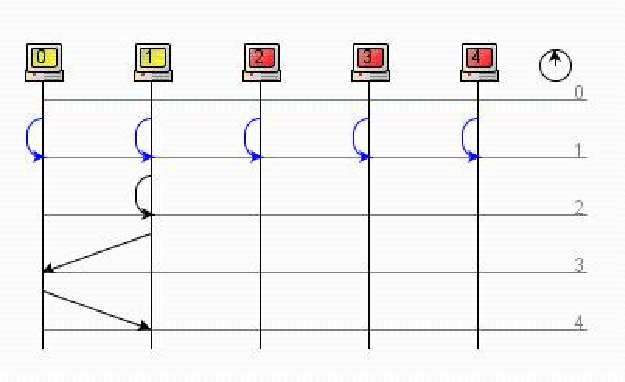
\includegraphics{images/p1ReadSeq.pdf}
    \caption{Skizzierung einer Faltungsoperation.}
    \label{fig-faltung}
    \small
    In dem Beispiel werden 4x4 grosse Daten zu 3x2 grossen feature maps ``gefaltet``.
\end{figure}



CNNs nutzen neben den Convolution Schichten auch Pooling Schichten [Ert21:325], die die Ausgaben des Netzes durch eine ``statistische Größe der nahegelegenen Ausgaben`` ersetzt [GBC18:379], was die Zahl der Pixel auf den feature maps reduziert\footnote{ \textit{LeCun, Bengio und Hinton} weisen in [LBH15:439] darauf hin, dass die Pooling Schicht auch die Aufgabe hat, semantisch ähnliche Merkmale zusammenzufassen: ``the role of the pooling layer is to merge semantically similar features into one.``
}, ausserdem wird als Aktivierungsfunktion meistens die nichtlineare ReLu (Rectified Linear Unit, s. Gleichung~\ref{eq:gl-relu} und Abbildung~\ref{fig-relu}) verwendet, die die Konvergenz der Netze verbessert [Ert21:327].\\

ReLU:
\begin{equation} f(x) = max(0, x)
    \label{eq:gl-relu}
\end{equation}


\begin{figure}[h]
    \centering
    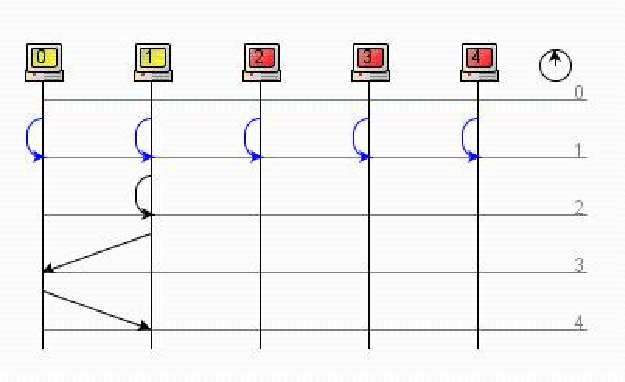
\includegraphics{images/p1ReadSeq.pdf}
    \caption{Ein Plot der ReLU}
    \label{fig-relu}
\end{figure}




